\section{Multilagen-PVD}
\label{multilayer}

Mit PVD-Methoden werden auch mehrlagige Schichten abgeschieden, die im folgenden Kapitel am Beispiel von dünnen Cu/Ni-Multilagen näher untersucht werden sollen.
Das Kupfer-Nickel-System wurde aufgrund ähnlicher Gitterkonstanten der elementaren Kristalle gewählt (Ni: \SI{3.52}{\angstrom}, Cu: \SI{3.61}{\angstrom}), die kristallines Wachstum ermöglichen und somit Fehlstellen unterbinden.
Durch die Ähnlichkeit zur Kupfer-PVD kann man zudem auf den dort entwickelten Prozessparametern und den untersuchten Potentialparametersätzen aufbauen.

Im Experiment werden mehrlagige Kupfer-Nickel-Schichten per Elektro\-deposition\cite{yang_pulsed_1995} oder durch Sputtern\cite{cammarata_nanoindentation_1990} hergestellt, wobei üblicherweise Lagendicken im Bereich mehrerer Nanometer erzielt werden.
Dieses Vorgehen lässt sich direkt in Parsivald-Simulationen übertragen, in denen zugunsten der Rechenzeit in den folgenden Untersuchungen vergleichsweise dünne Lagen mit einer Dicke von \SI{1}{\nano\meter} abgeschieden wurden.
Anschließend werden diese auf Ähnlichkeit mit LAMMPS-präparierten Multilagen hinsichtlich ihrer Lagendicke und -rauheit untersucht.
Eine Auswertung der relativen Verteilung der Spezies entlang der Abscheidungsrichtung wird ergänzend für verschiedene Relaxationszeiten als Maß der Lagenqualität durchgeführt.
Abscheidungen von Lagen mit einer Dicke von \SI{6}{\nano\meter} wurden ebenfalls mit Parsivald simuliert, doch mangels verfügbarer Rechenzeit für vergleichbare LAMMPS-Simulationen nicht eingehender untersucht.

Wie bei den Gold-PVD-Simulation zuvor müssen für erfolgreiche Simulationen einige Prozessparameter wie Relaxationszeit, Thermostatdämpfung und Substrattemperatur optimiert werden.
\todo{Wort}Das geschah hinsichtlich der Rauheit der Oberfläche zur Vermeidung von Fehlstellen sowie \todo{hinsichtlich hinsichtlich hinsichtlich}hinsichtlich der Qualität der einzelnen Lagen im Vergleich mit ähnlichen Untersuchungen\cite{zhou_atomistic_1998}.
In diesen wurde bereits gezeigt, dass die kinetische Energie der einfallenden Atome einen erheblichen Einfluss auf die Qualität der einzelnen Lagen hat, weshalb gleichartige Untersuchungen nur hinsichtlich der Substrattemperatur durchgeführt wurden.

\subsection{Ergebnisse}

Parsivald-Simulationen erzeugen nach korrekter Parametereinstellung monokristallin gewachsene, klar abgegrenzte Atomlagen geringer Rauheit, die sich gut mit den Ergebnissen gleichartiger LAMMPS-Simulationen decken (Abbildung \ref{fig:multilayerresults}).
Rauheitswerte um \SI{1.2}{\angstrom} stellen sich mit beiden Simulationsmethoden bis zur zehnten Lage ein und stimmen stimmen somit miteinander und mit den bisherigen Ergebnissen überein (Abbildung \ref{fig:multilayerplots-a}).

Zuvor war eine Anpassung der Temperaturen und Relaxationszeiten notwendig, die jedoch für LAMMPS und Parsivald gleichermaßen gelten.
Als Richtwert wurde die Qualität der einzelnen Lagen in Form des Anteils der Spezies in Abhängigkeit der Höhe über dem Substrat genutzt (Abbildung \ref{fig:multilayerplots-b}).
Lagen schlechterer Qualität zeigen eine höhere Durchmischung der Schichten, was wiederum zu einer Senkung der relativen Häufigkeit einer Spezies innerhalb ihrer Schicht führt, wie man für die beiden Verteilungen bei einer Relaxationszeit von \SI{0.2}{\femto\second} pro Ereignis beobachten kann.
Erst bei Verdopplung der Relaxationszeit bilden sich klar abgegrenzte Lagen aus, wie sie in Abbildung \ref{fig:multilayerresults} dargestellt sind.

In Anhang asd
\todo[inline]{Was ist im Anhang?}

\todo[inline]{ordentlich vorstellen!}

Bei größeren Systemen sind durch Verspannungen im Material Gitterversetzungen und -fehlstellen zu erwarten, die allerdings durch \todo{Wort}Finite-Size-Effekte unterdrückt sein können.

\begin{figure}
  \captionsetup[subfigure]{singlelinecheck=false}
  \def\subfigwidth{7cm}
  \begin{subfigure}[t]{\subfigwidth}
    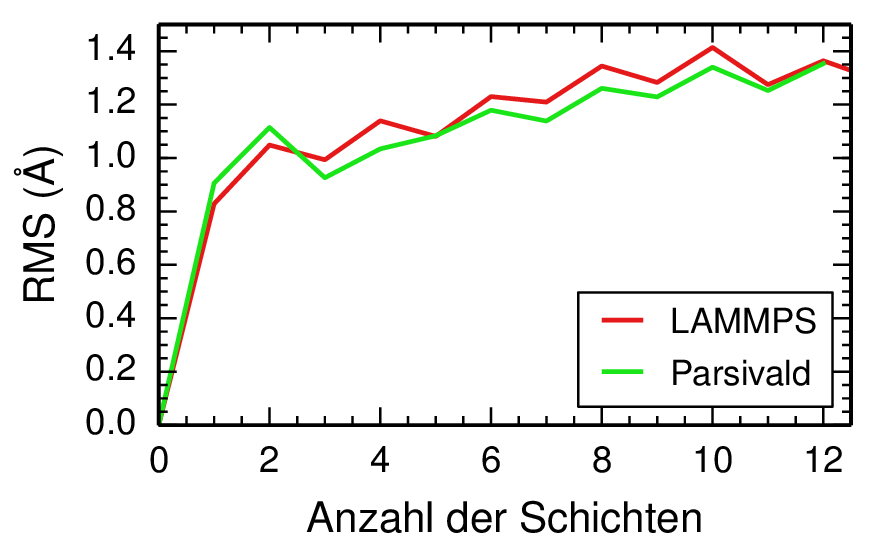
\includegraphics[width=\textwidth]{CuNi_layerroughness_comparison}
    \subcaption{
      Vergleich der Rauheit zwischen LAMMPS und Parsivald (Abb. \ref{fig:multilayerresults})
    }
    \label{fig:multilayerplots-a}
  \end{subfigure}
  \hfill
  \begin{subfigure}[t]{\subfigwidth}
    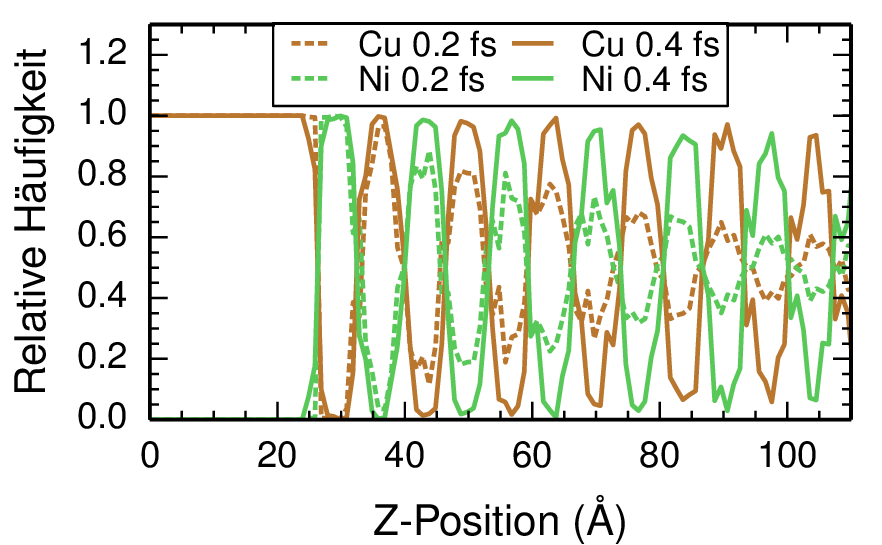
\includegraphics[width=\textwidth]{CuNi_atomdistribution_relax}
    \subcaption{Verteilung der Kupfer- und Nickelatome innerhalb der Schicht}
    \label{fig:multilayerplots-b}
  \end{subfigure}
  \caption[Ergebnisse der Multilagen-Abscheidung von Kupfer und Nickel]{
    Ergebnisse der Multilagen-Abscheidung von Kupfer und Nickel:
    Vergleich der zwischen LAMMPS und Parsivald (a) und Einfluss der Relaxationszeit auf die Schichtqualität in Parsivald (b)
  }
  \label{fig:multilayerplots}
\end{figure}

\begin{figure}
  \captionsetup[subfigure]{singlelinecheck=false}
  \def\subfigwidth{7cm}
  \begin{subfigure}[t]{\subfigwidth}
    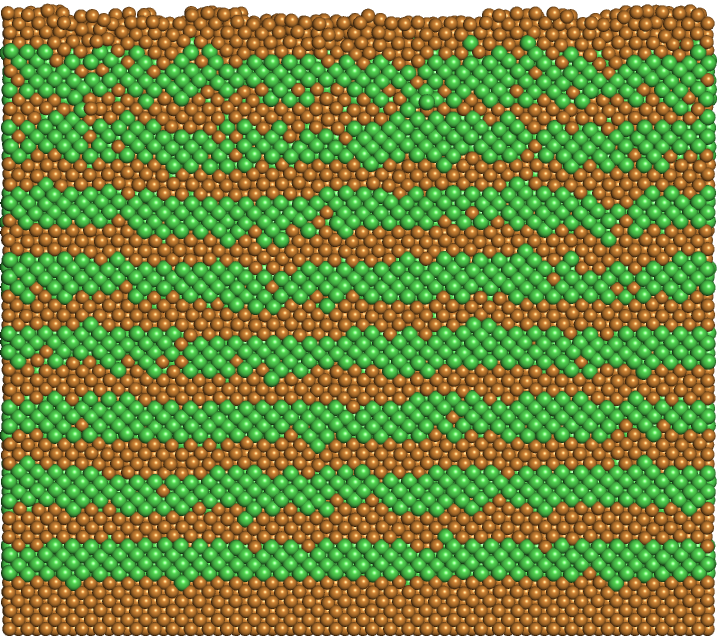
\includegraphics[width=\textwidth]{CuNi_profile_LAMMPS_nice}
    \subcaption{Profil einer per LAMMPS simulierten Multilagen-Abscheidung}
  \end{subfigure}
  \hfill
  \begin{subfigure}[t]{\subfigwidth}
    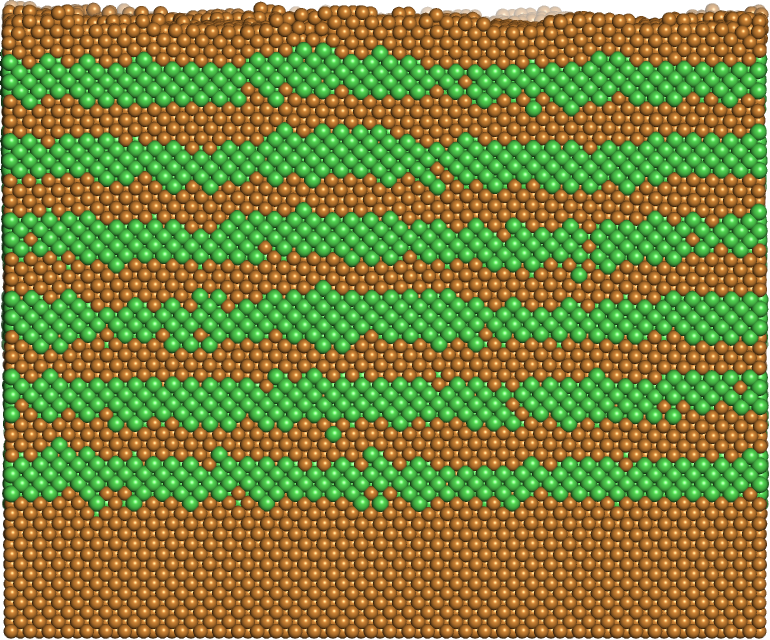
\includegraphics[width=\textwidth]{CuNi_profile_Parsivald}
    \subcaption{Profil einer per Parsivald simulierten Multilagen-Abscheidung}
  \end{subfigure}
  \caption[Vergleich zwischen Simulationen von Multilagensystemen mit Parsivald und LAMMPS]{
    Vergleich zwischen Simulationen von Multilagensystemen mit Parsivald und LAMMPS unter Nutzung optimierter Parameter.
  }
  \label{fig:multilayerresults}
\end{figure}
